\documentclass{article}
\usepackage{tikz}
\usepackage{xpatch}
\usetikzlibrary{shapes.geometric, arrows, positioning, fit, backgrounds}

% https://tex.stackexchange.com/a/562606/234654
\makeatletter
% similar to env "pgfonlayer", but the latest contents are typeset on
% lowest bottom (on reversed order)

\let\pgfonlayerreversed\pgfonlayer
\let\endpgfonlayerreversed\endpgfonlayer

\xpatchcmd\pgfonlayerreversed
  {\expandafter\box\csname pgf@layerbox@#1\endcsname\begingroup}
  {\begingroup}
  {}{\fail}

\xpatchcmd\endpgfonlayerreversed
  {\endgroup}
  {\endgroup\expandafter\box\csname pgf@layerbox@\pgfonlayer@name\endcsname}
  {}{\fail}


\tikzset{
  on background layer reversed/.style={%
    execute at begin scope={%
      \pgfonlayerreversed{background}%
      \let\tikz@options=\pgfutil@empty
      \tikzset{every on background layer/.try,#1}%
      \tikz@options
    },
    execute at end scope={\endpgfonlayerreversed}
  }
}


\def\StartDrawOnBottomOfLayerStack{%
  \scope\relax
  % patch \path variants to auto insert "\scoped[on lowest layer]"
  % currently \node, \pic, \coordinate, and \matrix are patched
  \let\tikz@path@overlay\tikz@path@overlay@autoscoped
  \let\tikz@path@overlayed\tikz@path@overlayed@autoscoped
}

\def\EndDrawOnTopOfLayerStack{%
  \endscope
}

\def\tikz@path@overlay@autoscoped#1{%
  \let\tikz@signal@path=\tikz@signal@path% for detection at begin of matrix cell
  \pgfutil@ifnextchar<%
    {\tikz@path@overlayed{#1}}
    {\scoped[on background layer reversed] \path #1}}%
\def\tikz@path@overlayed@autoscoped#1<#2>{%
  \scoped[on background layer reversed] \path<#2> #1}%
\makeatother

\begin{document}
\begin{figure}[h]
\centering
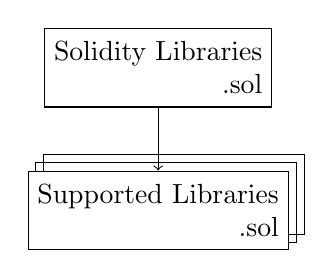
\begin{tikzpicture}
    \tikzset{rectangle node/.style={draw, minimum size=1cm}}

    \node[rectangle node, align=right] (sol) {Solidity Libraries \\.sol};

    \node[rectangle node, align=right,below=8mm of sol, fill=white] (solLib) {Supported Libraries \\.sol};

    \StartDrawOnBottomOfLayerStack
        \node [rectangle node, fit=(solLib), inner sep=0, xshift=1mm, yshift=1mm, fill=white] {};
        \node [rectangle node, fit=(solLib), inner sep=0, xshift=2mm, yshift=2mm] {};
    \EndDrawOnTopOfLayerStack

    \draw [->] (sol) -- (solLib);
    
\end{tikzpicture}
\caption{Code Generation Prozess}
\label{fig:CodeGenProzess}
\end{figure}
\end{document}